\section{Sieve Collimator and Blocker}

These collimators are only used during tracking measurements. They have the same deisign with the exception that the sieve collimator has strategically placed holes in order to sample specific scattering angles.

The primary purpose of the blocker is to block ``all'' of the charged particles that have scattered from the target and gone through the acceptance of the primary collimator to reach the main detectors. With the blocker in place, the main detectors (the thin quartz, and the shower-max detectors) should see \textit{none} of the M\o ller scattered electrons or e-p events from the hydrogen target. Any signal these detectors see should be due to background contributions. 

%rewrite this:
%~~~~~~~~~~~~~~~~~

This could include the so-called beam-line background (electrons scattered from the target at very small angles or from the halo in the beam that interacts with beam-line components, e.g. the inner bore of one of the collimators or the beam pipe itself which can then generate downstream, perhaps even past the spectrometer magnets) and could generate signal in the main detectors. 

%add citation for QWeak?
Such a background was important for the QWeak experiment. Details on this issue for MOLLER are given in ~\cite{beamlinebackground}. During MOLLER, we will use the blocker in integrating mode at normal (65 $\mu$A) beam current to measure and/or put upper limits on the signal amplitude (yield) and asymmetry of such a background. Backgrounds coming to the main detectors from the beam dump will also be part of this background. We will also use the blocker at lower beam currents in counting mode to measure pulse-height spectrum in the main detectors of these background events and see if they are associated with trackable charged particles using the GEMs. 

Any punch-through in the blocker coming from the target would need to be estimated from simulation and then verified in the counting mode using the GEMs and the trigger scintillators. Then, that contribution subtracted from the blocker-in data will be used to get the ``true'' beamline background. So the blocker needs to be placed in the beamline with the full beam current on the hydrogen target at 11 GeV beam energy. We may decide to run it with the 12C or Al targets as well if we ever do asymmetry measurements on those targets (i.e. transverse asymmetry or BNSSA measurements).

%~~~~~~~~~~~~~~~~~

% Move this to a later part!
The System Requirements document for the spectrometer system, which includes the blocker and sieve collimator, requires that the blocker be able to dissipate 1.4 kW of heating power. The mechanical design for the sieve and blocker were presented here:~\cite{bessuille}.

\subsection{Thickness}

The thickness of the blocker and the sieve are assumed to be the same, but if results require, their thicknesses can be different. They are the same!!! Include pictures!

The results from the blocker will be more sensitive to charged particles punching through the blocker and reaching the main detector, so it was used as our benchmark in simulation to define the requirements for the dimensions of our tracking system collimators. Our ultimate goal for the blocker is to see $\leq0.1\%$ signal of charged particles with the blocker in place compared to the signal without the blocker. For M\o ller scattered electrons, this requirement would be on the main detector's ring 5 ($950\leq r\leq1100$ mm) especially, and for e-p scattered electrons we will focus on the main detector's ring 2 ($690\leq r\leq750$ mm). %check these radii values

Our main method for analyzing thickness requirements was to look at the amount of ``punch-through'', the quantity of particles that entered the upstream surface of the blocker and exited the downstream surface of the blocker with enough energy to make it to the main detector, for given thicknesses. We analyzed punch-through of charged particles (electrons and positrons), primaries (the two M\o ller scattered electrons), and gammas separately. A starting point for the thickness was based on the radiation length of pure tungsten. Radiation length is an intrinsic value for a material, and it characterizes the amount of energy lost as electrons travel through the material. Approximately, for every unit of radiation length, the electron loses $1/3$ of its energy. Initially, the sieve and blocker were designed with 118mm thick pure tungsten (radiation length 3.5mm), which meant we could expect the electron to have $\sim(8.5\times10^{-13})\%$ of its original energy when it left the sieve or blocker. %double check this value

We originally wanted to investigate the sieve and blocker thickness to see if we could reasonably make them thinner. A thinner sieve and blocker would allow for more room on the beamline and would obviously cost less in material. When we analyzed the punch-through on the main detector, we mostly looked at charged particles that hit the main detector for any event in which a charged particle hit the upstream surface of the sieve or blocker. This is not \emph{true} punch-through, because it also includes charged particles that are from showers in the sieve, but it is still a useful benchmark because showers should be expected and accounted for. 

%Define earlier and better
In this paper, this is how ``punch-through'' will be defined. ``True punch-through'' will be defined as particles that traveled through the sieve from surface to surface.

The first method we used to analyze punch-through was to flag particles that hit the sieve sectors at the upstream surface but did not hit the sieve holes. We then only analyzed events that satisfied this condition.

\begin{figure}[H]
    \centering
    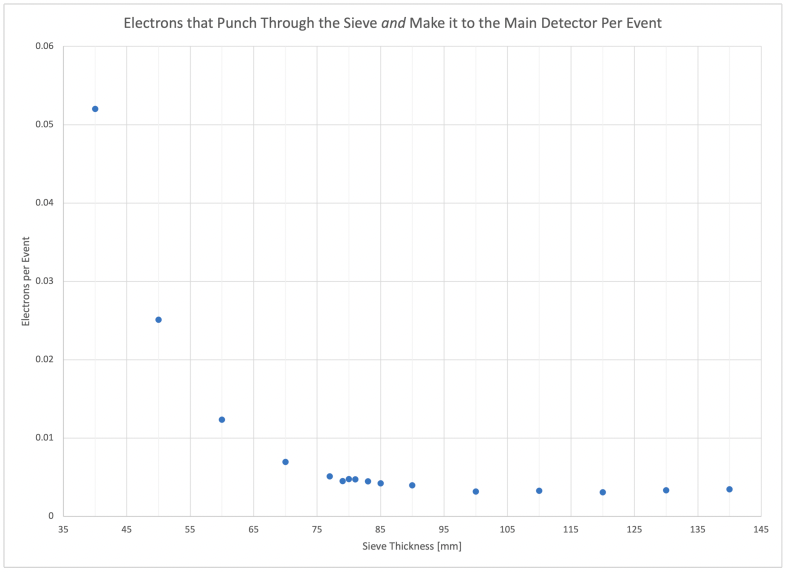
\includegraphics[scale=0.5]{Images/PunchThroughPerEvent_09082021.png}
    \caption{The number of punch-through electrons on the main detector weighted by number of events thrown plotted versus sieve thickness. This was made using the elasticC12 generator with a pure tungsten sieve and 5-pass beam energy.}
    \label{fig:sieve_electron_punchthrough}
\end{figure}

On Figure \ref{fig:sieve_electron_punchthrough}, there is a clear ``knee'' in the plot around a sieve thickness of $\sim85$mm. Figure \ref{fig:sieve_electron_punchthrough_zoom} shows the same plot zoomed in on this knee with error bars included. Thus, increasing the thickness past 85mm won't increase the effectiveness in stopping punch-through. However, there are a few more details to consider. Just because the knee in the plot is at 85mm doesn't mean we can't use a thinner sieve. 

\begin{figure}[H]
    \centering
    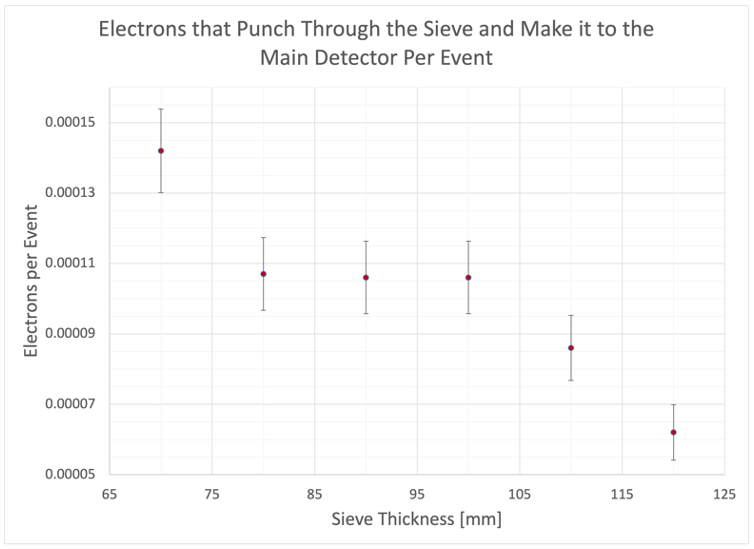
\includegraphics[scale=0.4]{Images/PunchThroughPerEvent_ErrorBars_09162021.png}
    \caption{The number of punch-through electrons on the main detector weighted by number of events thrown plotted versus sieve thickness. This was made using the elasticC12 generator with a pure tungsten sieve and 5-pass beam energy.}
    \label{fig:sieve_electron_punchthrough_zoom}
\end{figure}

If a sieve thickness of only 70mm, for example, yields a noise to signal ratio of approximately $0.1\%$ on the detector ring of interest, then that is a viable option. If this noise to signal ratio changes greatly at thicknesses less than 85mm, then we want to be conservative and pick a thickness slightly greater than 85mm to allow for uncertainty in machinery. As said earlier, the noise to signal ratio is less important for the sieve than it is for the blocker, but it's still important that this ratio be very small. Figure \ref{fig:sieve_noise_total} shows a similar ratio of interest that allows us to analyze the sieve thickness. The next plot of interest that could be made would be the same ratio on ring 2, which is where the eP scattered electrons should hit the main detector. Making this radial cut would focus in on the signal from the sieve holes that we don't want diluted by punch-through.

\begin{figure}[H]
    \centering
    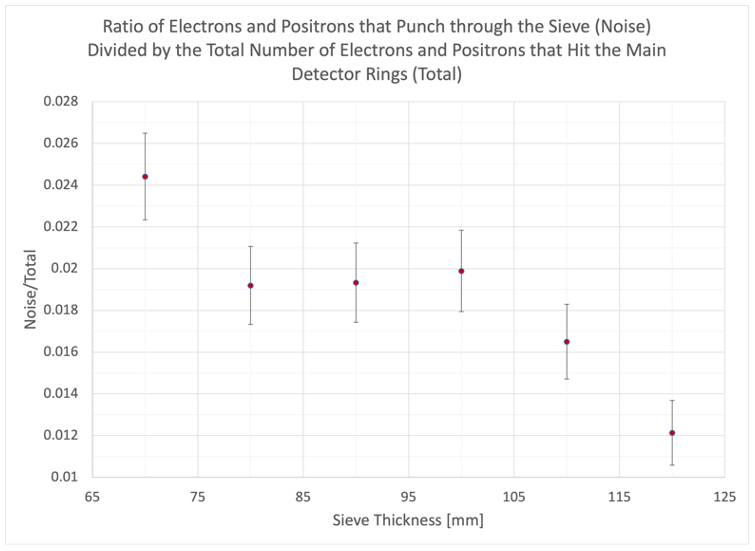
\includegraphics[scale=0.4]{Images/RatioNoiseToTotal_09162021.png}
    \caption{The number of punch-through electrons on the main detector divided by the total number of electrons versus sieve thickness. This was made using the elasticC12 generator with a pure tungsten sieve and 5-pass beam energy.}
    \label{fig:sieve_noise_total}
\end{figure}

Another limiting factor has to do with the sieve hole size, which will be discussed later. From an engineering standpoint, drilling a small hole into a thick piece of material is difficult. Specifically, we are held to the following standard:
\begin{equation}
    20\geq\frac{l}{d}\nonumber
\end{equation}
where $l$ is the sieve thickness and $d$ is the sieve hole diameter. If we are able to make the sieve thinner, we can make smaller holes. Restrictions on hole size will allow us to later reevaluate how thin we make the sieve.

After we looked at the sieve, we switched to analyzing the blocker. This was a much easier analysis because we didn't need to write any logic in the script to account for the sieve holes. We looked at the same plots but with the blocker in place instead of the sieve. Figure \ref{fig:CP_blocker_main} shows results using a pure tungsten blocker.

\begin{figure}[H]
    \centering
    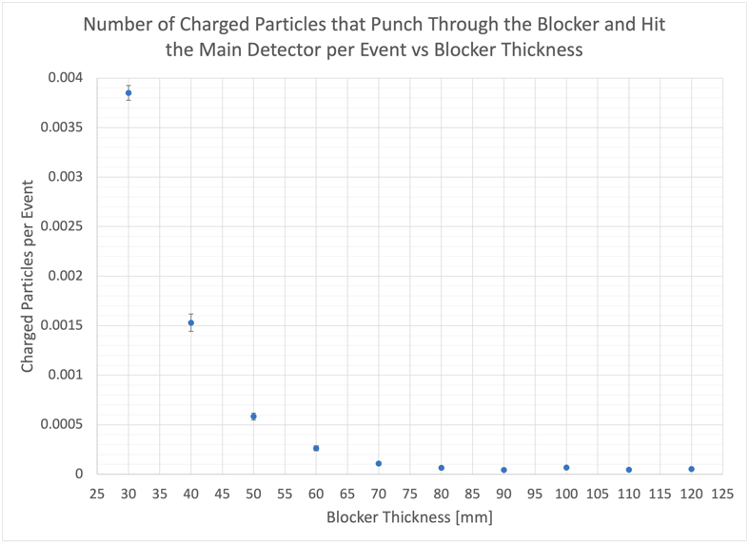
\includegraphics[scale=0.4]{Images/ChargedParticlesPunchThroughMainDet_Blocker_10062021.png}
    \caption{The number of punch-through charged particles on the main detector wieghted by the number of events thrown versus blocker thickness. This was made using the elasticC12 generator with a pure tungsten sieve and 5-pass beam energy.}
    \label{fig:CP_blocker_main}
\end{figure}

We also analyzed the number of punch-through charged particles divided by the total number of charged particles on the main detector. With the blocker in place, the ratio should be much larger because there are no sieve holes through which charged particles can travel. This is not the same as the noise over total ratio because we are looking at noise in both cases. Essentially we are analyzing how much of the noise on the main detector is due to punch through, so the ratio is punch-through noise over total noise. Figure \ref{fig:blocker_CP_main_ratio} shows how this ratio evolves with blocker thickness. There is clearly still a knee at roughly 85mm.

\begin{figure}[H]
    \centering
    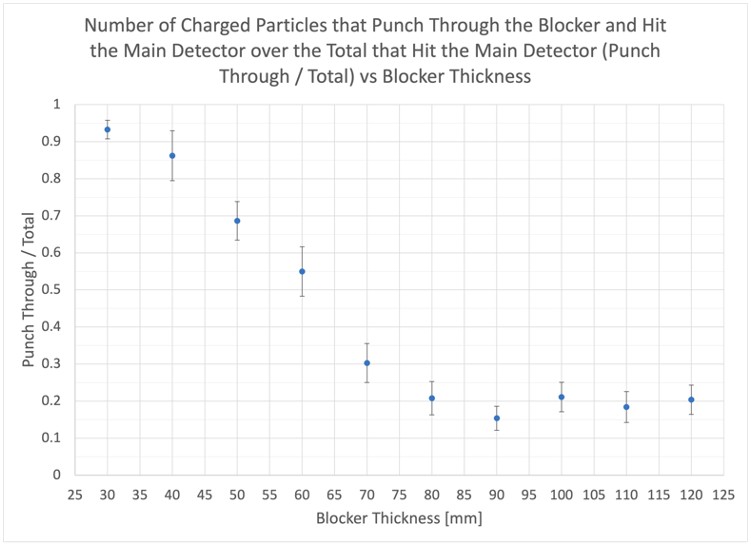
\includegraphics[scale=0.4]{Images/ChargedParticlesPunchThroughOverTotal_Blocker_10062021.png}
    \caption{The number of punch-through charged particles on the main detector divided by the total number of electrons versus blocker thickness. This was made using the elasticC12 generator with a pure tungsten sieve and 5-pass beam energy.}
    \label{fig:blocker_CP_main_ratio}
\end{figure}

We looked at the same results for gammas as well. Figure \ref{fig:blocker_main_gammas} shows that there is a knee at a slightly larger blocker thickness, roughly 110mm, but we are less concerned with this knee. Looking at gammas allows us to estimate the signal from photons, but as long as the signal is sufficiently small, we don't need to worry about it. The contribution of punch-through gammas to noise increases less than $10\%$ from blocker thickness 110mm to 85mm.

\begin{figure}[H]
    \centering
    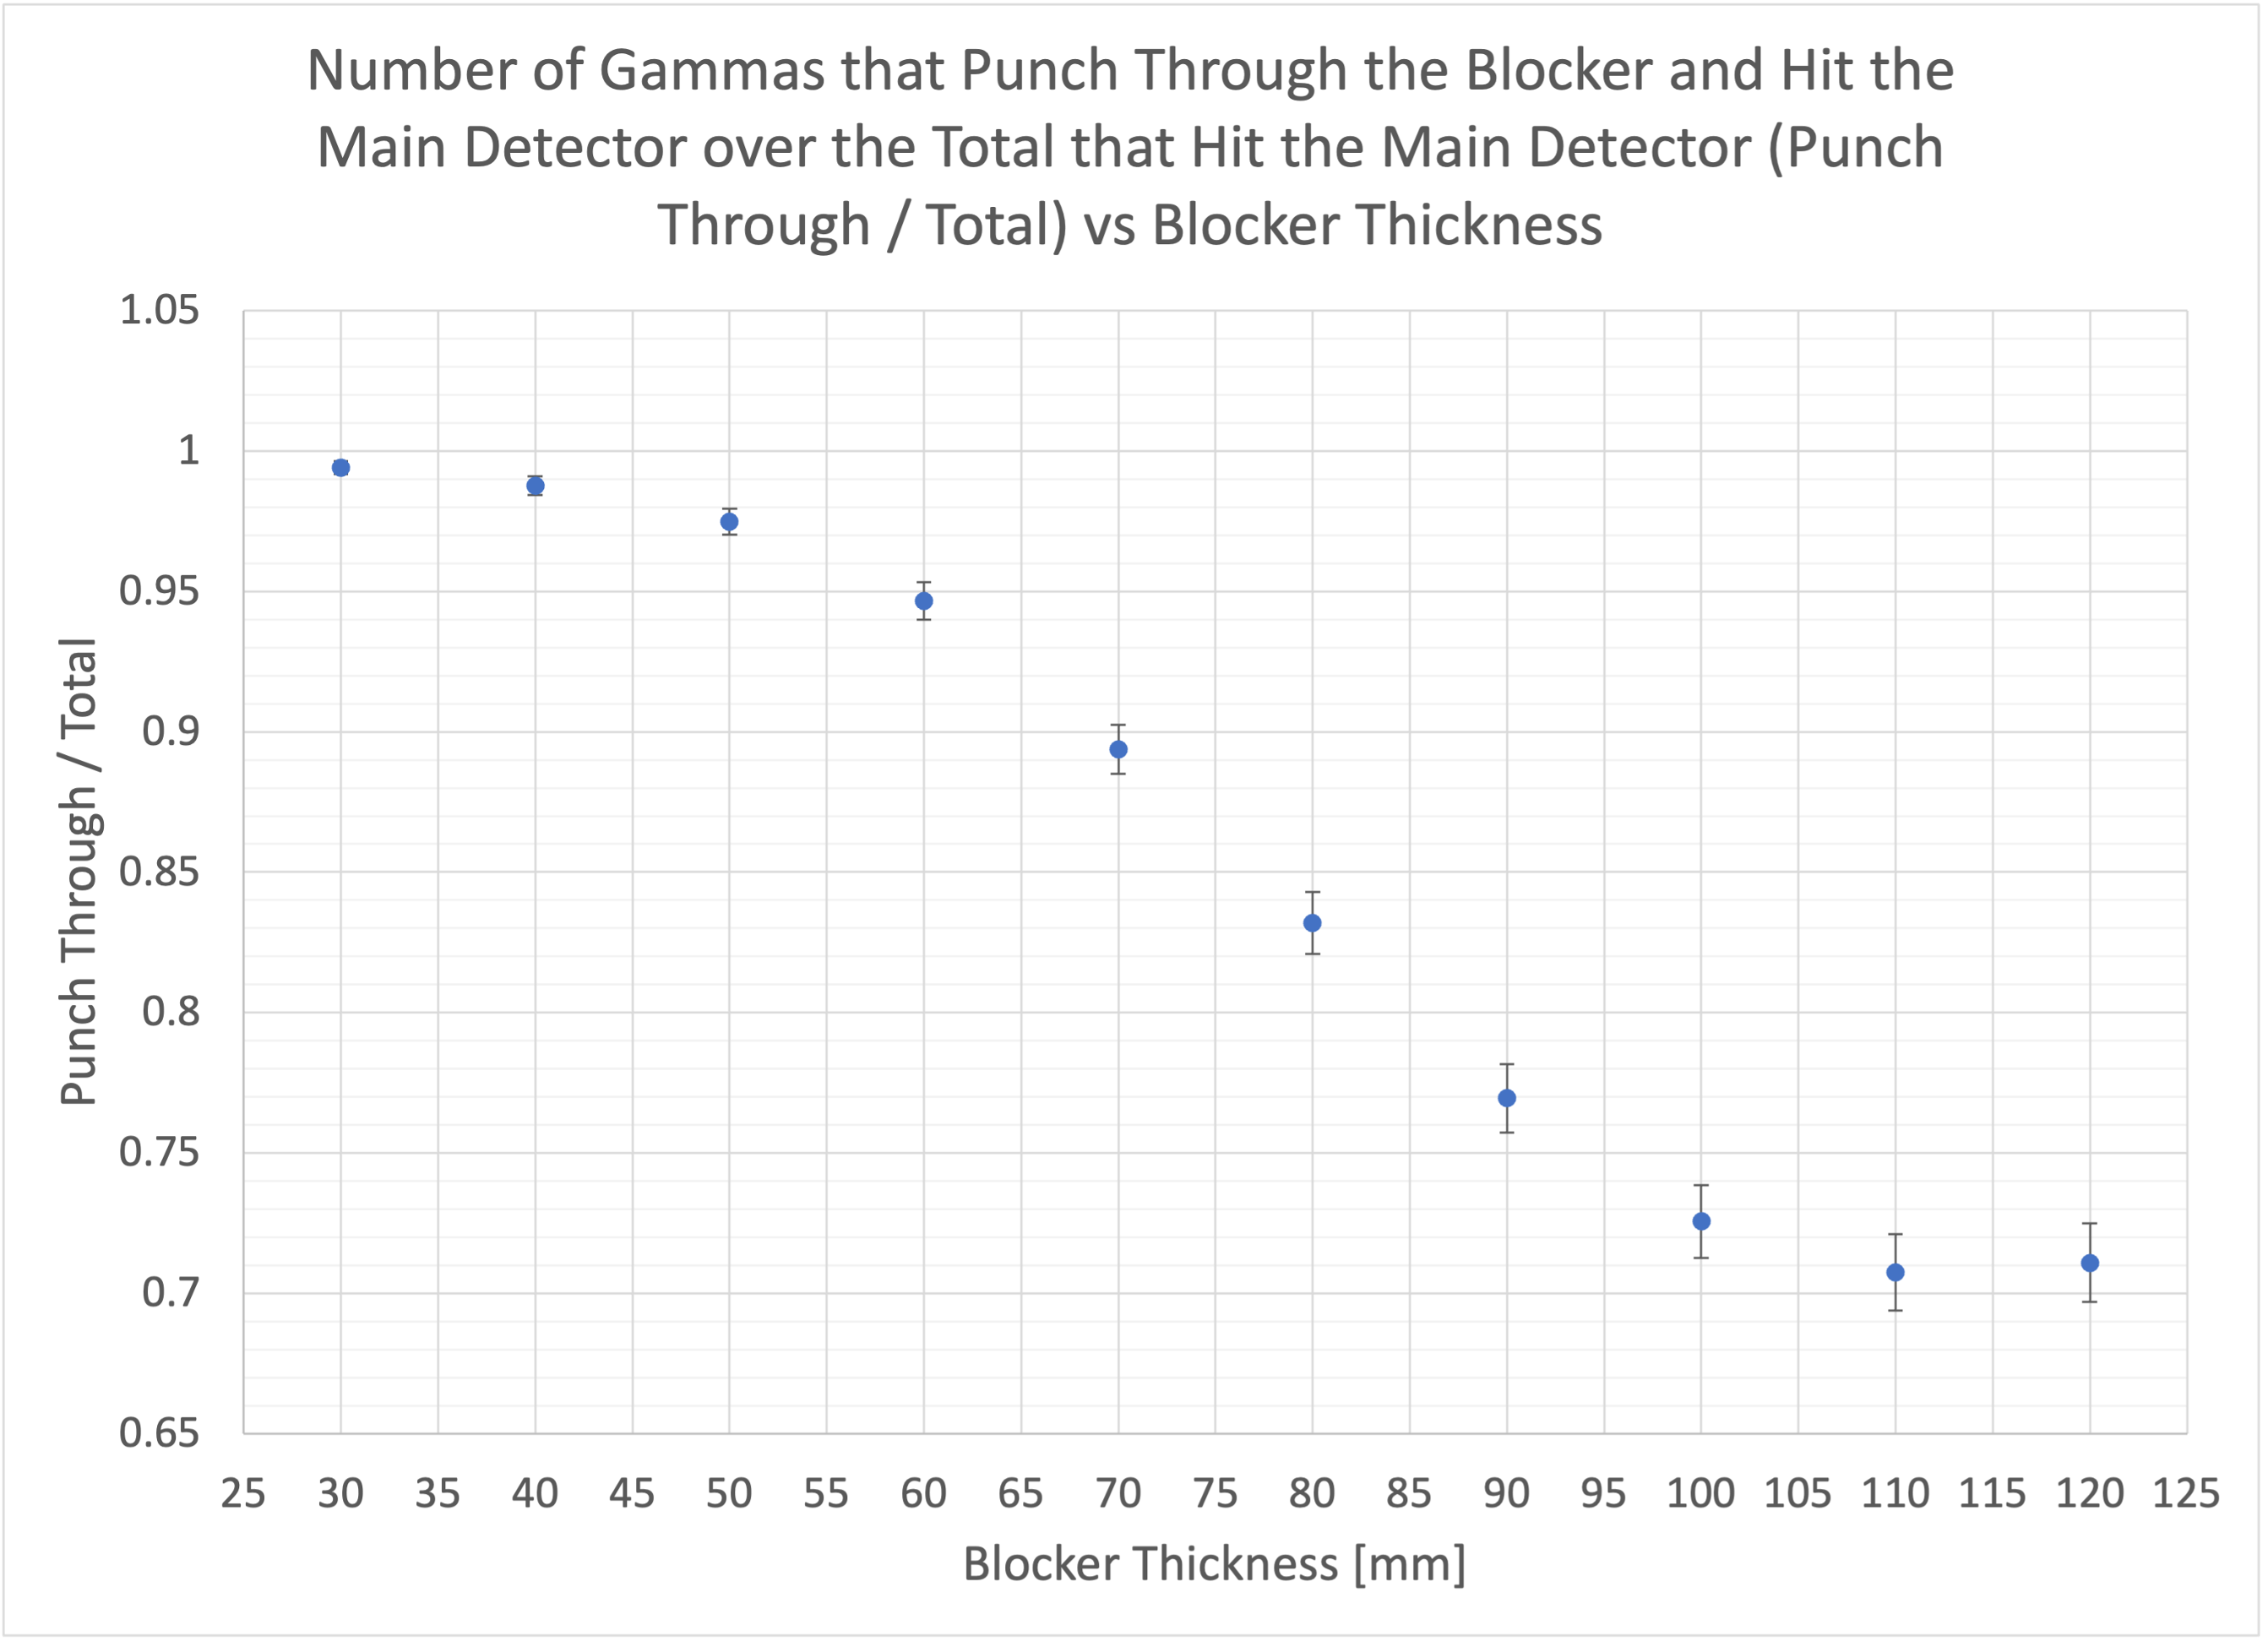
\includegraphics[scale=0.5]{Images/GammasPunchThroughOverTotal_Blocker_10202021.png}
    \caption{The number of punch-through charged gammas on the main detector divided by the total number of gammas versus blocker thickness. This was made using the elasticC12 generator with a pure tungsten sieve and 5-pass beam energy.}
    \label{fig:blocker_main_gammas}
\end{figure}

At this point in the study, we decided that a sieve and blocker thickness of 90mm was sufficient. We briefly revisited this study when we changed the sieve and blocker material (see Section 2.3).

\subsection{Inner Bore}

While initially analyzing the blocker thickness, we found an unexpected singularity on the main detector. When using the elesticC12 generator, one expects charged particles to be concentrated at $r\approx700$mm on the main detector because the magnet system bends e-p scattered electrons to that location. With the blocker in place, there should be no higher intensity signal at this radial location on the main detector because particles blocked by the blocker will be at a different energy then when they originally scattered, and the magnet will bend them differently. 

However, as shown in Figure \ref{fig:coll2_image} there is a clear signal of eP scattered electrons. This implied that some electrons were not being blocked at all. We will refer to these areas of unexpected high intensity on the main detector as ``acceptance images" because they appear at the azimuthal locations of the main acceptance.

\begin{figure}[H]
    \centering
    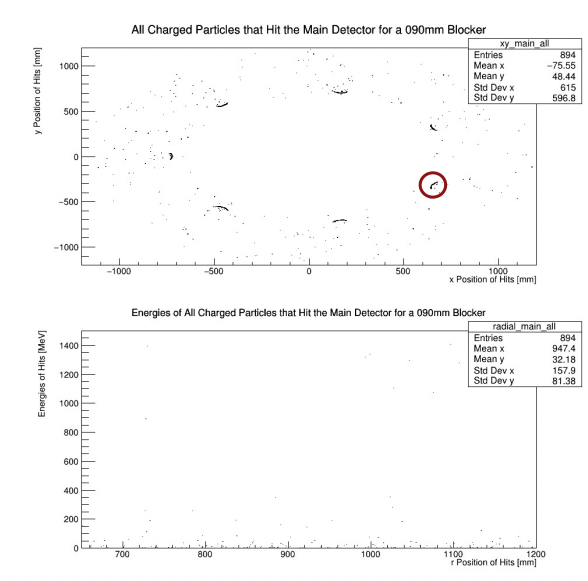
\includegraphics[scale=0.5]{Images/CharegedParticlesMainDetColl2Image_Blocker_10202021.png}
    \caption{Charged particles on the main detector with a 90mm pure tungsten blocker in place. This was made using the elasticC12 generator and 5-pass beam energy. The eP scattered electrons are circled on the top plot.}
    \label{fig:coll2_image}
\end{figure}

Our main hypothesis for the cause of these acceptance images was that the inner bore of the blocker allowed scattered particles through to the main acceptance collimator and the blocker inner radius needed to be changed. We thought that some combination of tapering the inner bore and making it smaller should allow us to fully block all of the scattered particles. A large factor to this idea was that the inner bore radius of the sieve and blocker was 35.3mm by default, and the inner radius of the main acceptance of collimator 2 was 35mm. Geometrically it would make sense that particles could enter the inner bore of the blocker and still be able to pass through collimator 2's acceptance.

The first step was to do a quick, informal test to see if reducing the inner bore radius would reduce the intensity of the acceptance images. Collimator 2 is roughly 500mm downstream of the blocker, so quick math said that 29mm should be a safe inner bore to try first. We also tried taking the smaller inner bore radius and tapering it by $0.5^{\circ}$ which is within the range of accepted scattering angles. We used a 50mm blocker to test this because we'd see more charged particles on the main detector for a thinner blocker. Figure \ref{fig:35mm_innerbore_50mmthick_blocker} shows the control results on the main detector. The acceptance images are clearly visible.

With a smaller inner bore radius, Figures \ref{fig:blocker_50mmthick_29mminnerbore_notaper} and \ref{fig:blocker_50mmthick_29mminnerbore_taper} clearly show that the acceptance images on the main detector disappear. However, comparing these two plots does not show a substantial difference when the inner bore is tapered. The downstream inner bore radius of the blocker is important to keep small when tapering. This means that when the inner bore is tapered, the upstream surface of the blocker gets larger.

\begin{figure}[H]
    \centering
    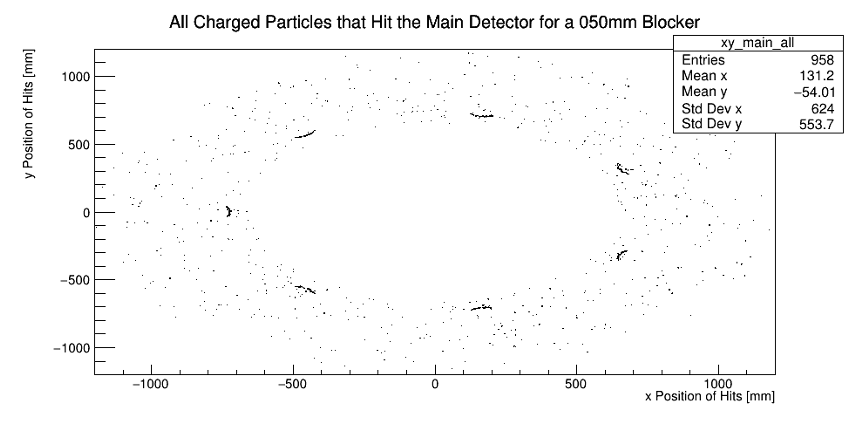
\includegraphics[scale=0.8]{Images/35mmInnerHoleCPMainDet.png}
    \caption{Charged particles on the main detector with a 50mm pure tungsten blocker in place. This was made using the elasticC12 generator and 5-pass beam energy.}
    \label{fig:35mm_innerbore_50mmthick_blocker}
\end{figure}

\begin{figure}[H]
    \centering
    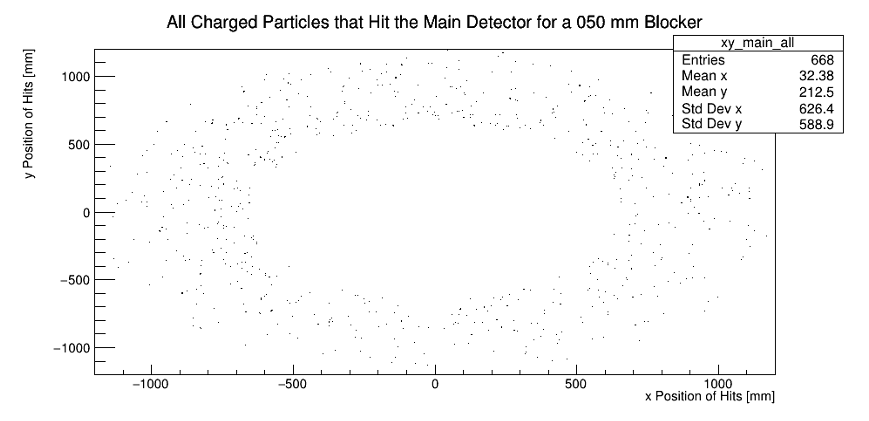
\includegraphics[scale=0.75]{Images/LessThan35mmWithNOTaperInnerHoleCPMainDet_12012021.png}
    \caption{Charged particles on the main detector with a 50mm pure tungsten blocker (29mm inner bore) in place. This was made using the elasticC12 generator and 5-pass beam energy.}
    \label{fig:blocker_50mmthick_29mminnerbore_notaper}
\end{figure}

\begin{figure}[H]
    \centering
    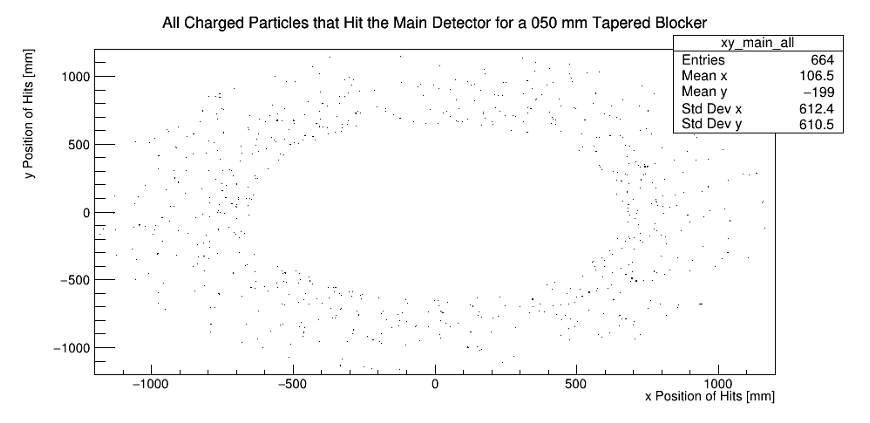
\includegraphics[scale=0.75]{Images/LessThan35mmWithTaperInnerHoleCPMainDet_12012021.png}
    \caption{Charged particles on the main detector with a 50mm pure tungsten blocker (29mm, $1.2^{\circ}$ taper inner bore) in place. This was made using the elasticC12 generator and 5-pass beam energy.}
    \label{fig:blocker_50mmthick_29mminnerbore_taper}
\end{figure}

These initial results showed us that an inner bore radius of 29mm was probably sufficient, but we wanted to look at this issue in more detail. If one draws out the geometry, as shown in Figure \ref{fig:innerBoreDrawing}, the largest acceptable inner bore radius (defined by the value $r=y_2-2.5\sqrt{2}$) should be 30.54mm. However, this number only accounts for the acceptance of collimator 2. There was some concern about slit scattering off of the edge of collimator 1 and into the acceptance of collimator 2. In order to account for this effect, the largest acceptable inner bore radius should be 28.63mm.

\begin{figure}[H]
    \centering
    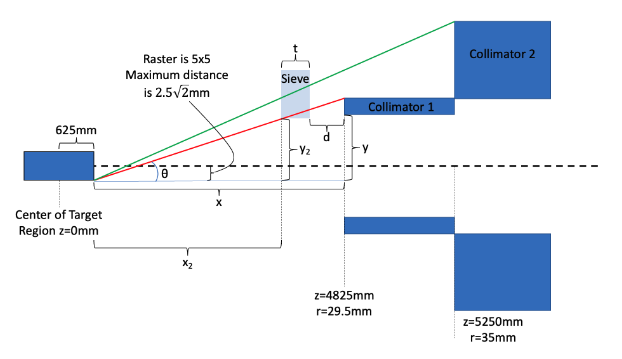
\includegraphics[width=\textwidth]{Images/InnerBoreGeometryDrawing.png}
    %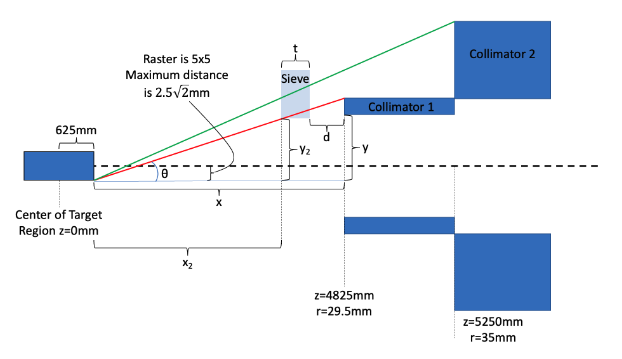
\includegraphics[scale=0.5]{Images/InnerBoreGeometryDrawing.png}
    \caption{Drawing used to calculate the inner bore of the blocker.}
    \label{fig:innerBoreDrawing}
\end{figure}

In order to quantitatively check if there was noticeable slit scattering from collimator 1, the first thing we did was make a vertex plot. This plot showed us the location in z that a charged particle on the main detector originated from. We were looking for vertices around 1000mm to indicate that particles were making it to the main detector from collimator 1. For a 50mm pure tungsten blocker, we got the following results:

\begin{figure}[H]
    \centering
    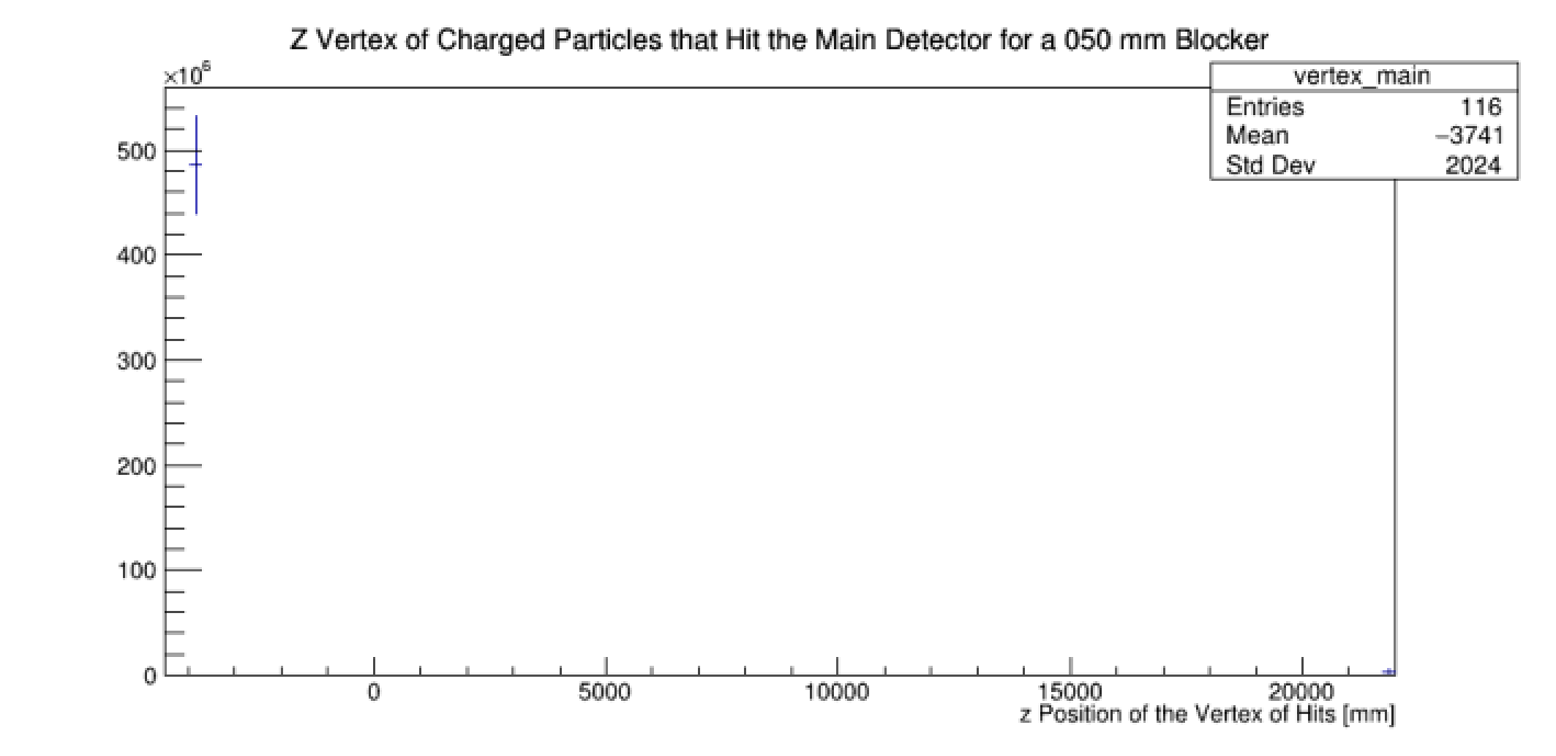
\includegraphics[width=\textwidth]{Images/VertexPlotCPMainDet50mmBlocker.png}
    \caption{This plot is made using hall center coordinates, so the target is located at $z=-4500$mm.}
    \label{fig:vertexblocker}
\end{figure}

Figure \ref{fig:vertexblocker} indicated that we do not see any slit scattering from collimator 1. This meant that we could allow for an inner bore radius of up to 30.54mm, but we felt that making the inner bore radius smaller was desirable. This would allow for uncertainty in the placement of the blocker in relation to collimators 1 and 2, and it would ensure that if collimator 1 slit scattering making it into the main acceptance is just an incredibly rare event, we could still protect ourselves from it.

A smaller inner bore radius means that more high energy particles will hit the blocker. Because of this, we needed to next confirm that the amount of power deposited on the blocker did not significantly change between a 30.54mm inner bore and a 28.63mm inner bore.

\subsection{Power Deposition}

For our power deposition study, we analyzed four different inner bore radii. We looked at 1mm, 26mm, 28.63mm, and 30.54mm. The small 1mm inner bore radius was used as a sanity check to ensure that the power deposition behaved as expected. With an inner bore that small, we expected to see an incredibly huge amount of power. We also used a more realistic 90mm thick pure tungsten blocker and a 5-pass 85$\mu$A beam.

\begin{figure}[H]
    \centering
    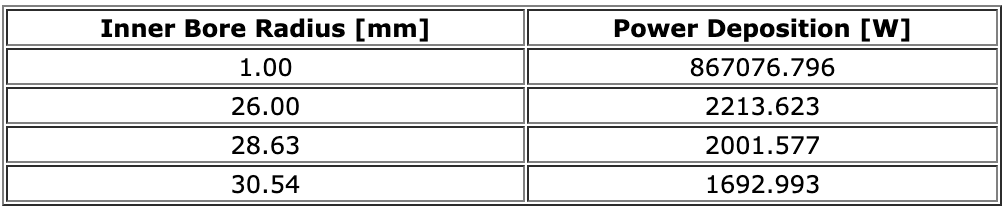
\includegraphics[width=\textwidth]{Images/PowerDepTable.png}
    \caption{Power deposition for 85$\mu$A of beam.}
    \label{fig:powerdeptable}
\end{figure}

Originally the sieve had been a petal design (Figure \ref{fig:segBlocker}) instead of a full cylinder (Figure \ref{fig:fullBlocker}), and we had to consider if designing the blocker as a petal was a good idea as well. It should make sense that if we used the petal design, the blocker saw about half of the power deposited onto it.

\begin{figure}
     \centering
     \begin{subfigure}[b]{0.45\textwidth}
         \centering
         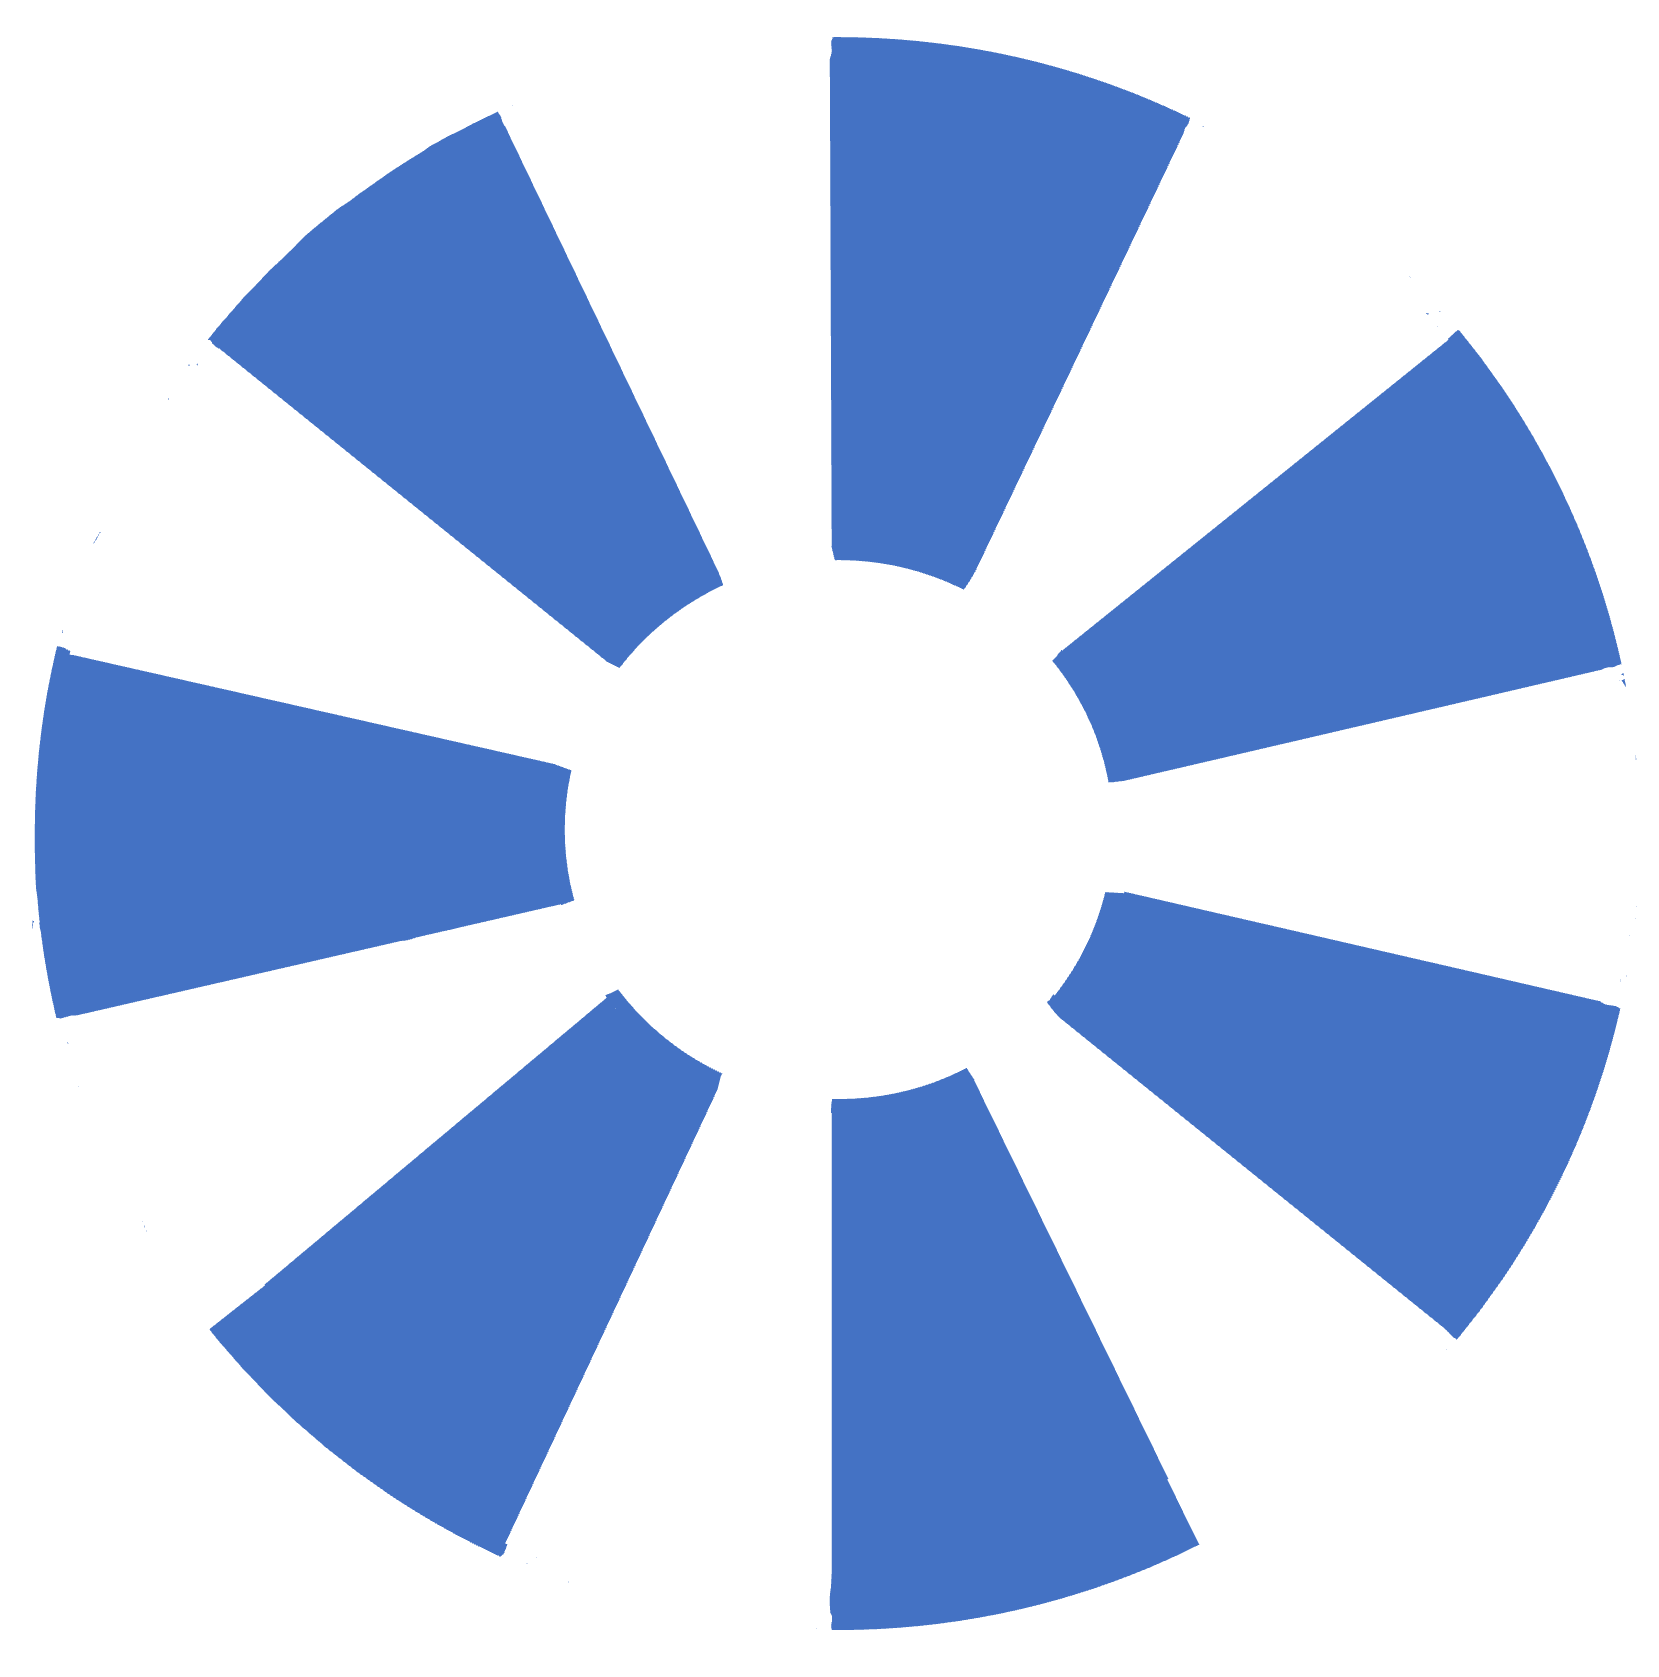
\includegraphics[width=\textwidth]{Images/SegBlocker.png}
         \caption{Segmented or ``petal" design}
         \label{fig:segBlocker}
     \end{subfigure}
     \hfill
     \begin{subfigure}[b]{0.45\textwidth}
         \centering
         
\includegraphics[width=\textwidth]{Images/FullBlocker.png}
         \caption{Full design}
         \label{fig:fullBlocker}
     \end{subfigure}
     \caption{Design Schemes for the Blocker}
     \label{fig:blockerDesigns}
\end{figure}

\subsection{Sieve Holes}

\subsubsection{Hole Placement}

\subsubsection{Hole Size}

\subsubsection{Hole Tilt}

